% Provenance (never printed): see sources/outline_sources.md and sources/book1/BRIEFS.md (g3/03).
\chapter{Files and Folders}\label{ch:g3:files-and-folders}

Leo wrote a poem last week, and today he wants to read it to the class. He
switches on the \omterm{def:g1:what-is-a-computer:computer}{computer} and looks at the \omterm{def:g2:using-a-computer:desktop}{desktop}: it is covered with forty
\omterm{def:g2:using-a-computer:desktop}{icons}, and most of them are called ``untitled''. He opens one: a drawing. He
opens another: a shopping list. The poem is somewhere in there, but where? It
takes him twenty minutes to find it. In this chapter, we see how the work kept
in a \omterm{def:g1:what-is-a-computer:computer}{computer} is organised, so that it can always be found again.

\begin{recall}
\omterm{def:g2:using-a-computer:save}{Saving} copies the work from the \omterm{def:g3:inside-the-computer:memory}{memory} into the \omterm{def:g3:inside-the-computer:storage}{storage}, where it is kept when
the power is off; a good name says what the work is
(\cref{ch:g2:using-a-computer,ch:g3:inside-the-computer}).
\end{recall}

\section{A file holds one piece of work}

\begin{definition}[File]\label{def:g3:files-and-folders:file}
A \emph{file}\index{file} is one piece of work kept in the \omterm{def:g3:inside-the-computer:storage}{storage} of a
\omterm{def:g1:what-is-a-computer:computer}{computer} under a name: a story, a drawing, a song, a film, a program. Its name
is the \emph{file name}\index{file name}.
\end{definition}

Every time you save a new piece of work, the \omterm{def:g1:what-is-a-computer:computer}{computer} makes a new \omterm{def:g3:files-and-folders:file}{file}. When you
open a \omterm{def:g3:files-and-folders:file}{file}, the \omterm{def:g1:what-is-a-computer:computer}{computer} copies it into the \omterm{def:g3:inside-the-computer:memory}{memory} so that you can see it and
change it; when you save again, the \omterm{def:g3:files-and-folders:file}{file} in the \omterm{def:g3:inside-the-computer:storage}{storage} is replaced by the new
version.

\section{Kinds of file and their extensions}

The name of a \omterm{def:g3:files-and-folders:file}{file} usually ends with a dot followed by a few letters:
\code{poem.txt}, \code{cat.jpg}, \code{song.mp3}.

\begin{definition}[Extension]\label{def:g3:files-and-folders:extension}
The \emph{extension}\index{extension (of a file name)} of a \omterm{def:g3:files-and-folders:file}{file name} is the
end of the name, after the last dot. It tells what kind of \omterm{def:g3:files-and-folders:file}{file} it is.
\end{definition}

\begin{center}
\begin{tabular}{ll}
\hline
\omterm{def:g3:files-and-folders:extension}{extension} & kind of \omterm{def:g3:files-and-folders:file}{file} \\
\hline
\code{.txt} & text, with no colours or styles \\
\code{.png}, \code{.jpg} & a picture \\
\code{.mp3} & a sound or a song \\
\code{.mp4} & a film \\
\code{.py} & a program written in Python \\
\hline
\end{tabular}
\end{center}

When you open a \omterm{def:g3:files-and-folders:file}{file}, the \omterm{def:g1:what-is-a-computer:computer}{computer} looks at its \omterm{def:g3:files-and-folders:extension}{extension} to choose a tool that
knows this kind of \omterm{def:g3:files-and-folders:file}{file}: a picture viewer for \code{.jpg}, a music player for
\code{.mp3}, a \omterm{def:g2:using-a-computer:word-processor}{text editor} for \code{.txt}. The \omterm{def:g3:files-and-folders:extension}{extension} is only a label: if
you change it, the inside of the \omterm{def:g3:files-and-folders:file}{file} stays exactly the same.

\begin{example}[A picture with the wrong label]\label{ex:g3:files-and-folders:label}
Sami renames \code{boat.png} to \code{boat.txt}. The \omterm{def:g3:files-and-folders:file}{file} still holds the same
picture, but now the \omterm{def:g1:what-is-a-computer:computer}{computer} opens it with the \omterm{def:g2:using-a-computer:word-processor}{text editor}, which shows a mess
of strange signs. When Sami gives back the name \code{boat.png}, the picture
opens again, unchanged.
\end{example}

A \omterm{def:g3:files-and-folders:file}{file} can also be made \emph{read-only}: it can then be opened and read, but
not changed. Later in this course, we see who is allowed to read or change
which \omterm{def:g3:files-and-folders:file}{files}.

\section{Folders inside folders}

\begin{definition}[Folder]\label{def:g3:files-and-folders:folder}
A \emph{folder}\index{folder} is a place in the \omterm{def:g3:inside-the-computer:storage}{storage}, with a name, that
holds \omterm{def:g3:files-and-folders:file}{files} and other folders.
\end{definition}

\begin{omfigure}
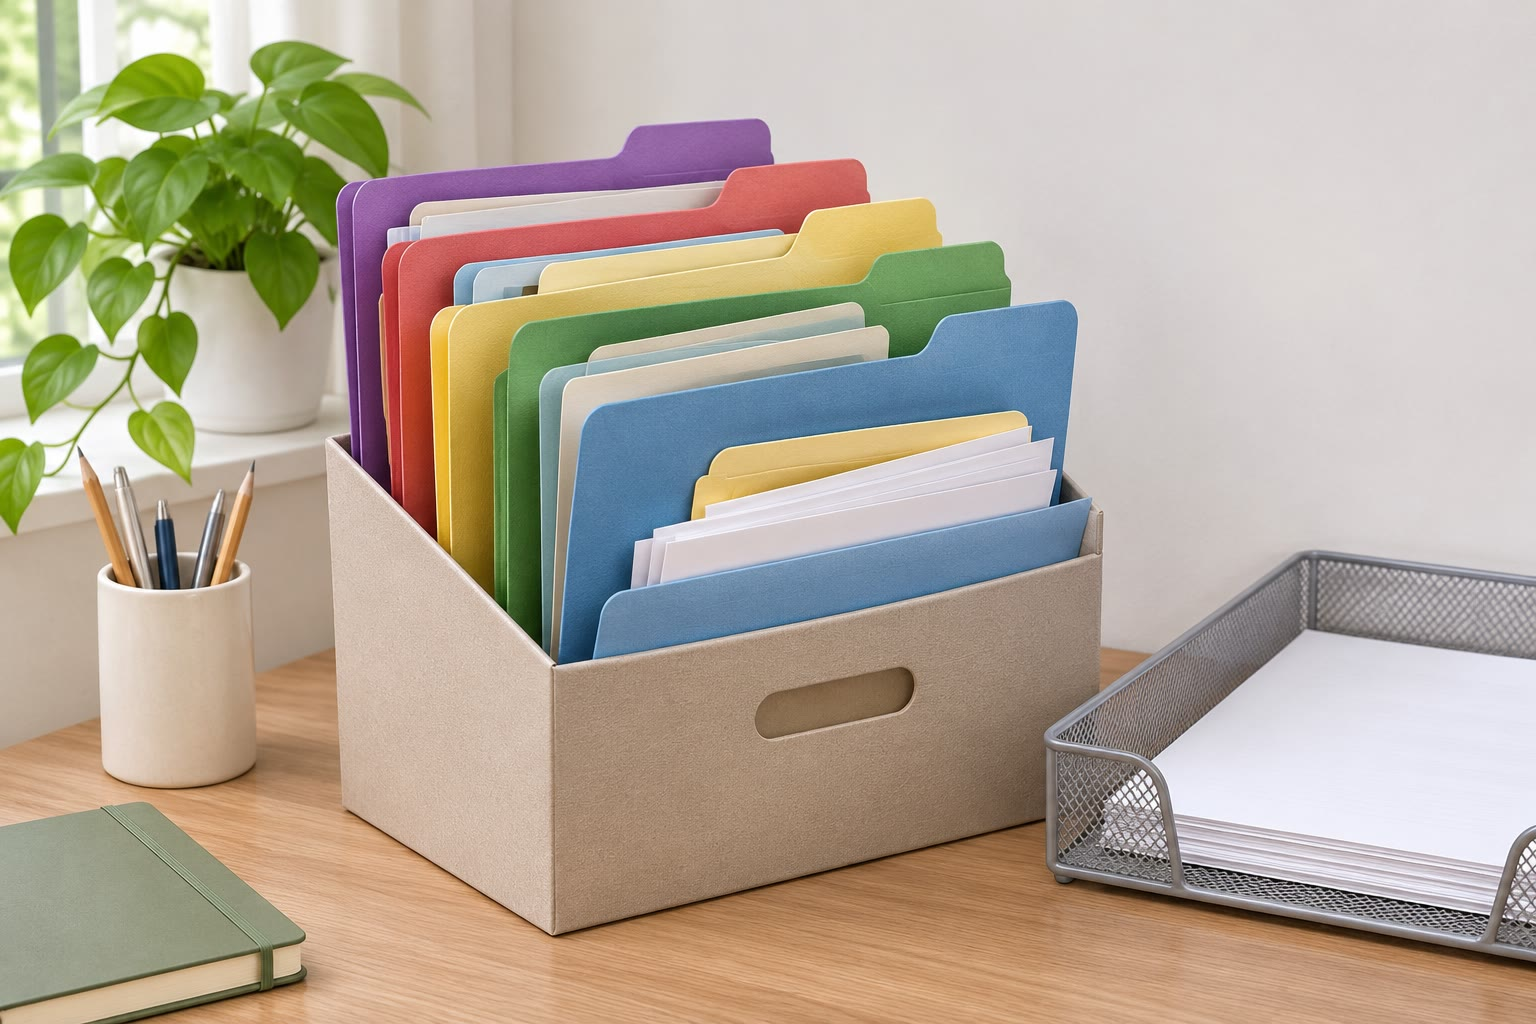
\includegraphics[width=0.48\linewidth]{images/book1/ai/g3-files-and-folders-desk.jpg}

{\small A tidy desk: papers in \omterm{def:g3:files-and-folders:folder}{folders}, \omterm{def:g3:files-and-folders:folder}{folders} in a box. A \omterm{def:g1:what-is-a-computer:computer}{computer} keeps its
\omterm{def:g3:files-and-folders:file}{files} the same way.}
\end{omfigure}

A \omterm{def:g3:files-and-folders:folder}{folder} can hold other \omterm{def:g3:files-and-folders:folder}{folders}, which can hold other \omterm{def:g3:files-and-folders:folder}{folders} again. Leo puts
his school work in a \omterm{def:g3:files-and-folders:folder}{folder} \code{School}, inside his \omterm{def:g3:files-and-folders:folder}{folder} \code{Documents};
inside \code{School}, there is a \omterm{def:g3:files-and-folders:folder}{folder} for each subject. All the \omterm{def:g3:files-and-folders:folder}{folders}
together, one inside the other, make a tree.

\begin{definition}[Folder tree]\label{def:g3:files-and-folders:tree}
The \emph{folder tree}\index{folder tree} of a \omterm{def:g1:what-is-a-computer:computer}{computer} is the drawing of all
its \omterm{def:g3:files-and-folders:folder}{folders} and \omterm{def:g3:files-and-folders:file}{files}, each one below the \omterm{def:g3:files-and-folders:folder}{folder} that holds it, with one \omterm{def:g3:files-and-folders:folder}{folder}
at the top that holds all the others.
\end{definition}

The \omterm{def:g3:files-and-folders:tree}{folder tree} is a tree drawn upside down: its root is at the top, and its
branches spread downwards. The \omterm{def:g3:files-and-folders:file}{files} are at the ends of the branches.

\begin{omfigure}
\begin{forest}
  for tree={font=\footnotesize\sffamily, draw=black!60, rounded corners=1.5pt,
    fill=ocYellow!40, inner sep=2.5pt, l sep=5mm, s sep=2.5mm, edge={black!50}},
  where n children=0{fill=white, font=\footnotesize\ttfamily}{},
  [Leo
    [Documents
      [School
        [Poems [poem.txt] [rain.txt]]
        [Maths [sums.txt]]]
      [letter.txt]]
    [Pictures [cat.jpg] [beach.png] [rocket.png]]
    [Music [song.mp3]]]
\end{forest}

{\small Leo's \omterm{def:g3:files-and-folders:tree}{folder tree}. The yellow boxes are \omterm{def:g3:files-and-folders:folder}{folders}, the white boxes are
\omterm{def:g3:files-and-folders:file}{files}.}
\label{fig:g3:files-and-folders:tree}
\end{omfigure}

\section{The path to a file}

To tell somebody where a \omterm{def:g3:files-and-folders:file}{file} is, we give the \omterm{def:g3:files-and-folders:folder}{folders} to open one after the
other, from the top of the tree down to the \omterm{def:g3:files-and-folders:file}{file}.

\begin{definition}[File path]\label{def:g3:files-and-folders:path}
The \emph{file path}\index{file path} of a \omterm{def:g3:files-and-folders:file}{file} is the list of the \omterm{def:g3:files-and-folders:folder}{folders}
from the top of the \omterm{def:g3:files-and-folders:tree}{folder tree} down to the \omterm{def:g3:files-and-folders:file}{file}, followed by the \omterm{def:g3:files-and-folders:file}{file name},
separated by the sign \code{/}.
\end{definition}

\begin{omfigure}
\begin{forest}
  for tree={font=\footnotesize\sffamily, draw=black!60, rounded corners=1.5pt,
    fill=ocYellow!40, inner sep=2.5pt, l sep=5mm, s sep=2.5mm, edge={black!50}},
  where n children=0{fill=white, font=\footnotesize\ttfamily}{},
  on path/.style={draw=ocRed!80!black, line width=1.2pt, edge={ocRed!80!black, line width=1.2pt}},
  [Leo, draw=ocRed!80!black, line width=1.2pt
    [Documents, on path
      [School, on path
        [Poems, on path [poem.txt, on path] [rain.txt]]
        [Maths [sums.txt]]]
      [letter.txt]]
    [Pictures [cat.jpg] [beach.png] [rocket.png]]
    [Music [song.mp3]]]
\end{forest}

\medskip
\code{Leo/Documents/School/Poems/poem.txt}

{\small The path to Leo's poem, from the top of the tree down to the \omterm{def:g3:files-and-folders:file}{file}.}
\label{fig:g3:files-and-folders:path}
\end{omfigure}

\begin{method}[Reading a path]\label{met:g3:files-and-folders:read-path}
Start at the \omterm{def:g3:files-and-folders:folder}{folder} at the top of the tree. Read the path from left to right:
each name before a \code{/} is a \omterm{def:g3:files-and-folders:folder}{folder} to open, inside the one before it. The
last name, after the last \code{/}, is the \omterm{def:g3:files-and-folders:file}{file}.
\end{method}

Most \omterm{def:g1:what-is-a-computer:computer}{computers} write the paths with \code{/}; some write them with the other
slant, \texttt{\textbackslash}. \omterm{def:g3:files-and-folders:file}{File} managers show the path of the open \omterm{def:g3:files-and-folders:folder}{folder}
at the top of their window.

\begin{omfigure}
\begin{tikzpicture}[font=\footnotesize]
  \omwindow{10}{4.4}{Pictures}
  \pic at (0,0) {window};
  \draw[black!50, fill=black!4, rounded corners=1pt] (0.25,3.35) rectangle (9.75,3.8);
  \node[anchor=west, font=\footnotesize\ttfamily] at (0.35,3.575) {Leo/Pictures};
  \node[anchor=east, font=\scriptsize, text=black!55] at (9.7,3.575) {the path of this folder};
  \foreach \x/\n/\c in {1.6/cat.jpg/ocYellow, 4.2/beach.png/ocBlue, 6.8/rocket.png/ocRed} {
    \draw[black!60, fill=white] (\x-0.55,1.25) rectangle (\x+0.55,2.85);
    \fill[\c!35] (\x-0.45,1.85) rectangle (\x+0.45,2.75);
    \draw[\c!70!black, thick] (\x-0.45,1.85) -- (\x-0.15,2.3) -- (\x+0.1,2.0) -- (\x+0.25,2.2) -- (\x+0.45,1.95);
    \fill[\c!70!black] (\x+0.25,2.55) circle (0.08);
    \node[font=\footnotesize\ttfamily] at (\x,0.85) {\n};
  }
\end{tikzpicture}

{\small A \omterm{def:g3:files-and-folders:file}{file} manager showing what is inside the \omterm{def:g3:files-and-folders:folder}{folder} \code{Pictures}: each
\omterm{def:g3:files-and-folders:file}{file} as an \omterm{def:g2:using-a-computer:desktop}{icon}, with its name and \omterm{def:g3:files-and-folders:extension}{extension} below it.}
\label{fig:g3:files-and-folders:manager}
\end{omfigure}

\section{Copying, moving, renaming, deleting}

\begin{definition}[Copy and move]\label{def:g3:files-and-folders:copy-move}
To \emph{copy}\index{copy (a file)} a \omterm{def:g3:files-and-folders:file}{file} into a \omterm{def:g3:files-and-folders:folder}{folder} is to make a second
\omterm{def:g3:files-and-folders:file}{file}, the same as the first, in that \omterm{def:g3:files-and-folders:folder}{folder}: then there are two. To
\emph{move}\index{move (a file)} a \omterm{def:g3:files-and-folders:file}{file} into a \omterm{def:g3:files-and-folders:folder}{folder} is to take it out of its
\omterm{def:g3:files-and-folders:folder}{folder} and put it in the other one: there is still only one.
\end{definition}

\begin{omfigure}
\begin{tikzpicture}[font=\footnotesize,
    fold/.style={draw=black!60, fill=ocYellow!40, rounded corners=1.5pt, font=\footnotesize\sffamily, minimum width=1.7cm, inner sep=2.5pt},
    fil/.style={draw=black!60, fill=white, rounded corners=1.5pt, font=\footnotesize\ttfamily, inner sep=2.5pt}]
  \foreach \x/\t/\l/\r in {0/before/1/0, 4.6/after copying/1/1, 9.2/after moving/0/1} {
    \node[font=\small\bfseries] at (\x+1.6,2.2) {\t};
    \node[fold] (a) at (\x+0.6,1.2) {Poems};
    \node[fold] (b) at (\x+2.6,1.2) {Best};
    \ifnum\l=1 \node[fil] (fa) at (\x+0.6,0) {poem.txt}; \draw[black!50] (a) -- (fa); \fi
    \ifnum\r=1 \node[fil] (fb) at (\x+2.6,0) {poem.txt}; \draw[black!50] (b) -- (fb); \fi
  }
  \draw[black!30] (4.1,-0.4) -- (4.1,2.4) (8.7,-0.4) -- (8.7,2.4);
\end{tikzpicture}

{\small Leo copies his poem into the \omterm{def:g3:files-and-folders:folder}{folder} \code{Best}: now there are two
poems. If he moves it instead, the poem leaves \code{Poems}: there is still
only one.}
\label{fig:g3:files-and-folders:copy-move}
\end{omfigure}

To \emph{rename} a \omterm{def:g3:files-and-folders:file}{file} is to change its name; the \omterm{def:g3:files-and-folders:file}{file} stays where it is,
unchanged. In a \omterm{def:g3:files-and-folders:folder}{folder}, two \omterm{def:g3:files-and-folders:file}{files} can never have the same name, or the \omterm{def:g1:what-is-a-computer:computer}{computer}
would not know which one you mean.

\begin{definition}[Bin]\label{def:g3:files-and-folders:bin}
The \emph{bin}\index{bin (recycle bin)} is a special \omterm{def:g3:files-and-folders:folder}{folder} where deleted
\omterm{def:g3:files-and-folders:file}{files} go. A \omterm{def:g3:files-and-folders:file}{file} in the bin can still be put back where it was; once the bin is
emptied, its \omterm{def:g3:files-and-folders:file}{files} are gone for good.
\end{definition}

\begin{inpractice}[A folder plan]
Before saving, choose the \omterm{def:g3:files-and-folders:folder}{folder}. Make one \omterm{def:g3:files-and-folders:folder}{folder} per subject, or per project,
with a short, clear name; inside, give each \omterm{def:g3:files-and-folders:file}{file} a name that says what it is,
like \code{poem-the-rain.txt}. Empty the \omterm{def:g3:files-and-folders:bin}{bin} only when you are sure that
nothing in it is needed.
\end{inpractice}

\section{Exercises}

\begin{exercise}[$\star$]\label{exo:g3:files-and-folders:1}
What kind of \omterm{def:g3:files-and-folders:file}{file} is each one? \code{map.png}, \code{notes.txt},
\code{dance.mp4}, \code{game.py}, \code{song.mp3}, \code{photo.jpg},
\code{list.txt}, \code{film.mp4}.
\end{exercise}

\begin{exercise}[$\star$]\label{exo:g3:files-and-folders:2}
Write the path to the \omterm{def:g3:files-and-folders:file}{file} \code{sums.txt} in Leo's \omterm{def:g3:files-and-folders:tree}{folder tree}.
\end{exercise}

\begin{exercise}[$\star$]\label{exo:g3:files-and-folders:3}
Which \omterm{def:g3:files-and-folders:folder}{folder} holds the \omterm{def:g3:files-and-folders:file}{file} \code{Leo/Pictures/rocket.png}? And the \omterm{def:g3:files-and-folders:file}{file}
\code{Leo/Documents/letter.txt}?
\end{exercise}

\begin{exercise}[$\star$]\label{exo:g3:files-and-folders:4}
Copy or move? (a)~Mia puts her story on a \omterm{def:g3:inside-the-computer:memory}{memory} stick for her teacher, and
keeps it on her \omterm{def:g1:what-is-a-computer:computer}{computer} too. (b)~Tom saved a picture in the wrong \omterm{def:g3:files-and-folders:folder}{folder}.
(c)~Lina wants a spare copy of her work in another \omterm{def:g3:files-and-folders:folder}{folder}, just in case.
\end{exercise}

\begin{exercise}[$\star$]\label{exo:g3:files-and-folders:5}
Where does a \omterm{def:g3:files-and-folders:file}{file} go when you delete it? Can it come back?
\end{exercise}

\begin{exercise}[$\star$]\label{exo:g3:files-and-folders:6}
Draw the \omterm{def:g3:files-and-folders:tree}{folder tree}: the \omterm{def:g3:files-and-folders:folder}{folder} \code{Mia} holds two \omterm{def:g3:files-and-folders:folder}{folders},
\code{Drawings} and \code{Stories}; \code{Drawings} holds \code{cat.png}
and \code{house.png}; \code{Stories} holds \code{dragon.txt}.
\end{exercise}

\begin{exercise}[$\star$]\label{exo:g3:files-and-folders:7}
Make a \omterm{def:g3:files-and-folders:folder}{folder} plan for your school year: the \omterm{def:g3:files-and-folders:folder}{folders} you would create, and
where they would go in the tree.
\end{exercise}

\begin{exercise}[$\star$]\label{exo:g3:files-and-folders:8}
How many \omterm{def:g3:files-and-folders:folder}{folders} and how many \omterm{def:g3:files-and-folders:file}{files} are there in Leo's \omterm{def:g3:files-and-folders:tree}{folder tree}?
\end{exercise}

\begin{exercise}[$\star\star$]\label{exo:g3:files-and-folders:9}
Leo renames \code{poem.txt} to \code{poem.jpg}. What happens when he opens it?
Is his poem lost?
\end{exercise}

\begin{exercise}[$\star\star$]\label{exo:g3:files-and-folders:10}
Two \omterm{def:g3:files-and-folders:file}{files} called \code{notes.txt} can be kept in two different \omterm{def:g3:files-and-folders:folder}{folders}, but
not in the same \omterm{def:g3:files-and-folders:folder}{folder}. Why?
\end{exercise}

\begin{exercise}[$\star\star$]\label{exo:g3:files-and-folders:11}
On Sami's \omterm{def:g2:using-a-computer:desktop}{desktop} there are three \omterm{def:g3:files-and-folders:folder}{folders}, \code{Pictures}, \code{Writing}
and \code{Poems}, and three \omterm{def:g3:files-and-folders:file}{files}, \code{cat.jpg}, \code{dog.jpg} and
\code{story.txt}. He wants \code{Poems} and \code{story.txt} inside
\code{Writing}, and both pictures inside \code{Pictures}. Each move moves one
\omterm{def:g2:using-a-computer:desktop}{icon}, and a \omterm{def:g3:files-and-folders:folder}{folder} moves with everything inside it. What is the smallest
number of moves? Draw his tree afterwards.
\end{exercise}
